% ==================================================
% گزارش کامل پروژه خوانش کیوبیت
% ==================================================

\chapter{کاهش خطای خوانش کیوبیت با استفاده از یادگیری ماشین}

% =========================
\section*{چکیده}

در این پژوهش، مسئله‌ی پیش‌بینی حالت کامل یک سامانه‌ی چهار کیوبیتی بر اساس داده‌های خوانش کوادریچر مورد بررسی قرار گرفته است. داده‌ها شامل اندازه‌گیری‌های مختلط برای هر کیوبیت در فضای \(I,Q\) بوده و هدف، نگاشت هر نمونه‌ی اندازه‌گیری به یکی از ۱۶ حالت ممکن سامانه‌ی چهار کیوبیتی است. 

روش‌های مختلف یادگیری ماشین شامل مدل‌های تمایزی و مولد مورد بررسی قرار گرفتند. در این راستا، علاوه بر مدل‌های کلاسیک مانند \lr{SVM}، از رویکردهای مبتنی بر مدل‌سازی آماری نظیر \lr{QDA} و \lr{Gaussian Mixture Model} نیز استفاده شد. همچنین مهندسی ویژگی در قالب نمایش‌های مختلف داده و استفاده از کرنل‌های الهام‌گرفته از نگاشت‌های کوانتومی مانند \lr{ZZ feature map} مورد بررسی قرار گرفت.

نتایج نشان می‌دهد که دقت پیش‌بینی چندکلاسه در بهترین حالت به حدود ۳۹ درصد محدود شده است. تحلیل‌های انجام‌شده نشان می‌دهد که این محدودیت عمدتاً ناشی از هم‌پوشانی ذاتی توزیع‌های خوانش تک‌کیوبیتی است و نه ضعف مدل‌های یادگیری ماشین.

% =========================
\section{مقدمه}

خوانش حالت کیوبیت‌ها یکی از چالش‌های اساسی در سامانه‌های محاسبات کوانتومی است. در بسیاری از پلتفرم‌ها مانند کیوبیت‌های ابررسانا، خوانش در ناحیه‌ی \lr{dispersive regime} انجام می‌شود. در این حالت، وضعیت کیوبیت باعث ایجاد تغییر کوچکی در فرکانس تشدیدگر شده و این تغییر از طریق اندازه‌گیری سیگنال‌های کوادریچر استخراج می‌شود.

سیگنال‌های خوانش معمولاً به صورت نقاطی در صفحه‌ی مختلط \((I,Q)\) نمایش داده می‌شوند. به‌دلیل وجود نویز و محدودیت‌های فیزیکی سیستم، توزیع این نقاط برای حالت‌های مختلف کیوبیت‌ها دارای هم‌پوشانی قابل توجهی است که منجر به خطای خوانش می‌شود.

هدف این پروژه، طراحی و ارزیابی مدل‌هایی برای کاهش خطای خوانش و پیش‌بینی حالت کامل چهار کیوبیت به صورت:
\[
\ket{q_4 q_3 q_2 q_1}
\]

% =========================
\section{ساختار داده‌ها}

داده‌های مورد استفاده شامل ۱۶ فایل متنی با نام‌هایی از \lr{0000.txt} تا \lr{1111.txt} هستند. هر فایل متناظر با یک حالت چهارکیوبیتی خاص است. 

در هر فایل:
\begin{itemize}
	\item ۴ خط وجود دارد (هر خط مربوط به یک کیوبیت)
	\item هر خط شامل ۱۰۰۰ مقدار مختلط است
\end{itemize}

در نتیجه، مجموعه‌داده شامل ۱۶۰۰۰ نمونه است که هر نمونه دارای ۴ عدد مختلط به عنوان ویژگی ورودی و یک برچسب ۴ بیتی به عنوان خروجی می‌باشد.

% =========================
\subsection{بارگذاری و سازماندهی داده}

در این مرحله، داده‌ها از فایل‌های متنی خوانده شده و به یک ساختار مناسب برای پردازش تبدیل شدند. هر نمونه به صورت یک بردار شامل چهار عدد مختلط در نظر گرفته شد و برچسب آن از نام فایل استخراج گردید.

% >>>>>>>>>>>>>>>>>>>>>>>>>>>>>>>>>>>>
\textbf{کد مربوط به بارگذاری داده‌ها:}
\includepdf[pages=-]{jupyter_codes/code_data_loading.pdf}
% <<<<<<<<<<<<<<<<<<<<<<<<<<<<<<<<<<<<

% =========================
\section{تحلیل آماری اولیه}

برای درک ساختار داده‌ها، تحلیل‌های بصری مختلفی انجام شد. این تحلیل‌ها شامل ترسیم نمودارهای پراکندگی در صفحه‌ی \(I,Q\) و بررسی توزیع آماری داده‌ها بود.

\begin{figure}[h]
	\centering
	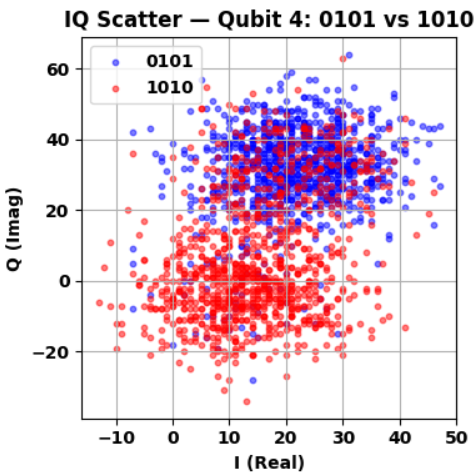
\includegraphics[width=0.7\linewidth]{figs/iq.png}
	\caption{نمونه‌ای از داده‌های خوانش در فضای \(I,Q\)}
\end{figure}

نتایج نشان داد که توزیع داده‌های مربوط به حالت‌های مختلف دارای هم‌پوشانی شدید هستند. حتی با تقریب گاوسی، بیضی‌های کوواریانس به‌شدت با یکدیگر تداخل دارند.

\begin{figure}[h]
	\centering
	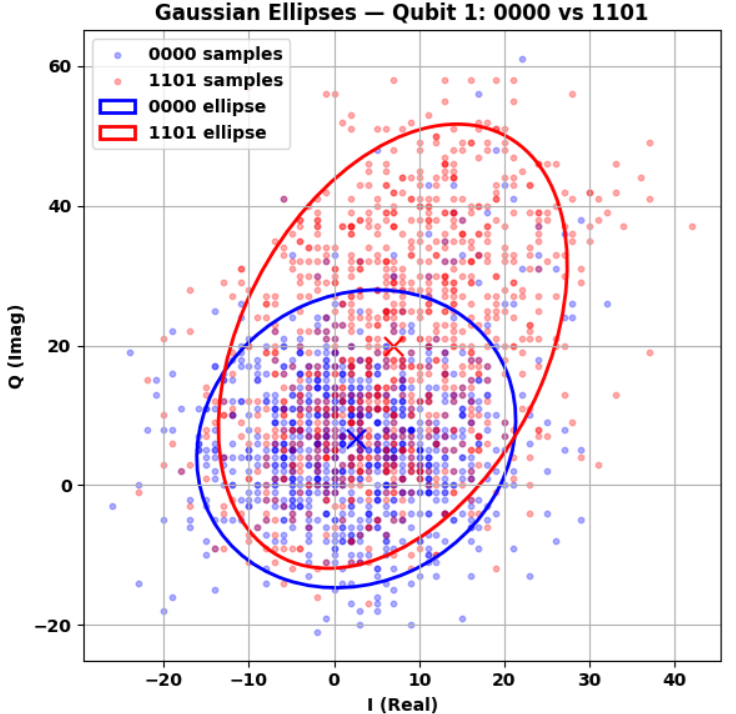
\includegraphics[width=0.8\linewidth]{figs/Gauss.png}
	\caption{تقریب گاوسی توزیع داده‌ها}
\end{figure}

این موضوع نشان می‌دهد که مسئله‌ی طبقه‌بندی ذاتاً دشوار است.

% >>>>>>>>>>>>>>>>>>>>>>>>>>>>>>>>>>>>
\textbf{کد تحلیل آماری و رسم نمودارها:}
\includepdf[pages=-]{jupyter_codes/code_visualization.pdf}
% <<<<<<<<<<<<<<<<<<<<<<<<<<<<<<<<<<<<

% =========================
\section{مهندسی ویژگی و پیش‌پردازش}

برای استفاده از داده‌های مختلط در مدل‌های یادگیری ماشین، دو نوع نمایش برای ویژگی‌ها در نظر گرفته شد.

\subsection{نمایش حقیقی-موهومی}
در این روش، هر عدد مختلط به دو مولفه‌ی حقیقی و موهومی تبدیل شد. بنابراین، بردار ویژگی هر نمونه دارای ۸ بعد خواهد بود.

\subsection{نمایش دامنه-فاز}
در این نمایش، هر عدد مختلط به دامنه و فاز آن تبدیل شد. این نمایش از نظر فیزیکی معنادارتر است.

\subsection{نرمال‌سازی داده‌ها}
برای بهبود عملکرد مدل‌ها، روش‌های مختلف نرمال‌سازی بررسی شد:
\begin{itemize}
	\item \lr{StandardScaler}
	\item \lr{RobustScaler}
\end{itemize}

نتایج نشان داد که \lr{RobustScaler} عملکرد بهتری در حضور نویز دارد.

% >>>>>>>>>>>>>>>>>>>>>>>>>>>>>>>>>>>>
\textbf{کد پیش‌پردازش و مهندسی ویژگی:}
\includepdf[pages=-]{jupyter_codes/code_preprocessing.pdf}
% <<<<<<<<<<<<<<<<<<<<<<<<<<<<<<<<<<<<

% =========================
\section{تحلیل جدایش‌پذیری تک‌کیوبیتی}

در این بخش، برای هر کیوبیت یک مدل طبقه‌بندی دودویی مستقل آموزش داده شد. هدف از این کار، تعیین سقف دقت قابل دستیابی بر اساس اطلاعات هر کیوبیت بود.

\begin{center}
	\begin{tabular}{c c}
		\hline
		کیوبیت & دقت \\
		\hline
		1 & 71.3\% \\
		2 & 81.8\% \\
		3 & 80.2\% \\
		4 & 81.4\% \\
		\hline
	\end{tabular}
\end{center}

اگر فرض شود که خطاهای کیوبیت‌ها مستقل هستند، دقت کل برابر خواهد بود با:
\[
0.713 \times 0.818 \times 0.802 \times 0.814 \approx 0.38
\]

این مقدار با دقت مشاهده‌شده در مدل چندکلاسه هم‌خوانی دارد.

% >>>>>>>>>>>>>>>>>>>>>>>>>>>>>>>>>>>>
\textbf{کد مدل تک‌کیوبیتی:}
\includepdf[pages=-]{jupyter_codes/code_single_qubit.pdf}
% <<<<<<<<<<<<<<<<<<<<<<<<<<<<<<<<<<<<

% =========================
\section{مدل‌سازی با \lr{SVM}}

مدل \lr{SVM} به عنوان مدل پایه مورد استفاده قرار گرفت.

\subsection{کرنل‌های استاندارد}
در ابتدا از کرنل \lr{RBF} استفاده شد که توانایی مدل‌سازی مرزهای غیرخطی را دارد.

\subsection{کرنل الهام‌گرفته از کوانتوم}
برای لحاظ کردن برهم‌کنش بین ویژگی‌ها، کرنل \lr{ZZ feature map} معرفی شد. این کرنل شامل ترم‌های جفتی از ویژگی‌ها است که به صورت توابع کسینوسی تعریف می‌شوند.

\begin{figure}[h]
	\centering
	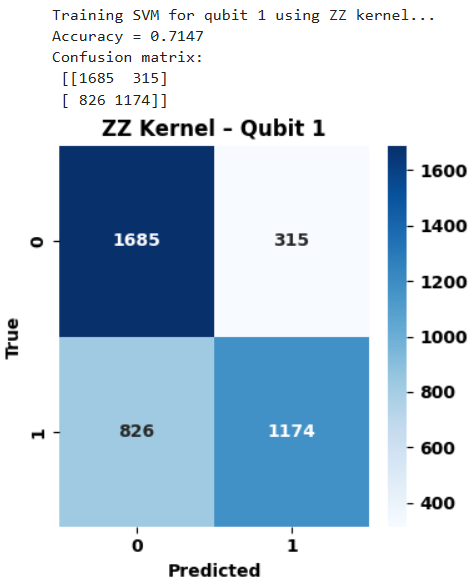
\includegraphics[width=0.6\linewidth]{figs/zz_kernel.png}
	\caption{نتایج کرنل ZZ}
\end{figure}

% >>>>>>>>>>>>>>>>>>>>>>>>>>>>>>>>>>>>
\textbf{کد SVM و کرنل ZZ:}
\includepdf[pages=-]{jupyter_codes/code_svm.pdf}
% <<<<<<<<<<<<<<<<<<<<<<<<<<<<<<<<<<<<

% =========================
\section{تحلیل وابستگی بین کیوبیت‌ها}

برای بررسی وجود \lr{cross-talk}، وابستگی بین خوانش کیوبیت‌ها بررسی شد. نتایج نشان داد که:

\begin{itemize}
	\item وابستگی اصلی روی قطر ماتریس است
	\item وابستگی بین‌کیوبیتی بسیار ضعیف است
\end{itemize}

بنابراین، محدودیت دقت ناشی از وابستگی بین کیوبیت‌ها نیست.

% >>>>>>>>>>>>>>>>>>>>>>>>>>>>>>>>>>>>
\textbf{کد تحلیل وابستگی:}
\includepdf[pages=-]{jupyter_codes/code_correlation.pdf}
% <<<<<<<<<<<<<<<<<<<<<<<<<<<<<<<<<<<<

% =========================
\section{مدل گاوسی بیزی (\lr{QDA})}

در این روش، فرض می‌شود که داده‌های هر کلاس از یک توزیع گاوسی چندمتغیره پیروی می‌کنند:

\[
x \sim \mathcal{N}(\mu_s, \Sigma_s)
\]

سپس با استفاده از قانون بیز، کلاس پیش‌بینی می‌شود.

برای بهبود عملکرد:
\begin{itemize}
	\item نرمال‌سازی داده‌ها انجام شد
	\item از \lr{shrinkage} برای کوواریانس استفاده شد
\end{itemize}

دقت نهایی:
\[
39.2\%
\]

% >>>>>>>>>>>>>>>>>>>>>>>>>>>>>>>>>>>>
\textbf{کد QDA:}
\includepdf[pages=-]{jupyter_codes/code_qda.pdf}
% <<<<<<<<<<<<<<<<<<<<<<<<<<<<<<<<<<<<

% =========================
\section{مدل مخلوط گاوسی (\lr{GMM})}

در این روش، هر کلاس به صورت ترکیبی از چند توزیع گاوسی مدل شد:

\[
P(x|s) = \sum \pi_k \mathcal{N}
\]

با افزایش تعداد مؤلفه‌ها، دقت کاهش یافت که نشان‌دهنده‌ی بیش‌برازش است.

% >>>>>>>>>>>>>>>>>>>>>>>>>>>>>>>>>>>>
\textbf{کد GMM:}
\includepdf[pages=-]{jupyter_codes/code_gmm.pdf}
% <<<<<<<<<<<<<<<<<<<<<<<<<<<<<<<<<<<<

% =========================
\section{بحث و تحلیل نهایی}

نتایج نشان می‌دهد که:
\begin{itemize}
	\item هم‌پوشانی توزیع‌ها عامل اصلی خطا است
	\item مدل‌ها به سقف اطلاعاتی رسیده‌اند
\end{itemize}

این موضوع نشان می‌دهد که بهبود بیشتر نیازمند تغییرات فیزیکی در سیستم است.

% =========================
\section{مسیرهای پیشنهادی}

\subsection{بهبودهای فیزیکی}
\begin{itemize}
	\item افزایش نسبت سیگنال به نویز
	\item بهبود تفکیک‌پذیری خوانش
\end{itemize}

\subsection{بهبودهای الگوریتمی}
\begin{itemize}
	\item استفاده از \lr{ensemble learning}
	\item استفاده از \lr{deep learning}
	\item استفاده از مدل‌های کوانتومی مانند \lr{QSVM}
\end{itemize}

% =========================
\section{جمع‌بندی}

در این پروژه، مسئله‌ی خوانش چهار کیوبیت بررسی شد و نشان داده شد که محدودیت اصلی دقت، ماهیت فیزیکی داده‌ها است. مدل‌های مختلف به سقف عملکرد خود رسیده‌اند و بهبود بیشتر نیازمند تغییر در فرآیند اندازه‌گیری است.